\documentclass[12pt,a4paper]{report}

\usepackage[cm]{fullpage}
\usepackage{paralist}
\usepackage{pdfpages}
\usepackage{graphicx}
\usepackage{wrapfig}
\usepackage{changepage}
\usepackage{scrextend}
\usepackage[nottoc,chapter]{tocbibind}
\newcommand{\HRule}{\rule{\linewidth}{0.5mm}}
\title{Workflow thing}

\author{Michiel Johan Baird \\
        Department of Computer Science \\
        University of Cape Town
    \\   \small{Supervisor: Dr. Hussein Suleman} }

\begin{document}
\begin{titlepage}

\begin{center}


% Upper part of the page
\includegraphics[width=0.15\textwidth]{./images/cslogo}\\[1cm]


\textsc{\Large Honours Project Report}\\[0.5cm]


% Title
\HRule \\[0.4cm]
{ \huge \bfseries Proposed Workflow System that meets the requirements of the Zamani Project}\\[0.4cm]

\HRule \\[1.5cm]

% Author and supervisor
\begin{minipage}{0.4\textwidth}
\begin{flushleft} \large
\emph{Author:}\\
Michiel Johan \textsc{Baird}
\end{flushleft}
\end{minipage}
\begin{minipage}{0.4\textwidth}
\begin{flushright} \large
\emph{Supervisor:} \\
Dr.~Hussein \textsc{Suleman}
\end{flushright}
\end{minipage}

% Bottom of the page
\vfill
\begin{table}[h]
\centering
\begin{tabular}{|l|p{7.5cm}|l|l|l|}
\hline
& \textbf{Category} & \textbf{Min} & \textbf{Max} & \textbf{Chosen} \\
\hline
1 & Requirements Analysis and Design & 0 & 20 & 15 \\
\hline
2 & Theoretical Analysis & 0 & 25 & 0 \\
\hline
3 & Experiment Design and Execution & 0 & 20 & 10 \\
\hline
4 & System Development and Implementation & 0 & 15 & 10 \\
\hline
5 & Results Findings and Conclusion & 10 & 20 & 10 \\
\hline
6 & Aim Formulation and Background Work & 10 & 15 & 10 \\
\hline
7 & Quality of Report Writing and Presentation &
\multicolumn{2}{|c|}{10}  & 10 \\
\hline
8 & Adherence to Project Proposal and Quality of Deliverables &
\multicolumn{2}{|c|}{10}  & 10 \\
\hline
9 & Overall General Project Evaluation & 0 & 10 & 5 \\
\hline
\multicolumn{2}{|l|}{\textbf{Total}} & \multicolumn{2}{|l|}{\textbf{80}} & \textbf{80} \\
\hline
\end{tabular}
\end{table}




\textsc{\Large University of Cape Town}\\[0.5cm]
\textsc{\Large Department of Computer Science}\\[0.5cm]
{\large \today} \\
\end{center}
\HRule \\[0.2cm]
{\raggedleft The financial assistance of the National Research Foundation (NRF) towards this research is hereby acknowledged. Opinions
expressed and conclusions arrived at, are those of the author and are not necessarily to be attributed to the NRF.}\\
\HRule \\[0.2cm]



\end{titlepage}

\pagenumbering{roman}
\begin{abstract}
Workflow Management Systems have been highly successful in managing complicated
tasks and procedures, both for business and scientific applications. This
research project follows the development of an \emph{Automatic Workflow System}
designed to meet the needs of the tasks that are present within the
\emph{Zamani Project}. This is developed to handle very large files, which is a
common within the project. The system was developed in three design iterations
built from the requirements and considerations of the group. A Web interface
is used to control the system. The system was built in Python using the \emph{Django}
framework along with JQuery and other front-end libraries.

Both automated and user tasks are supported in the system. For user tasks, the
required files are automatically copied to the user's workstation. This is done
using \emph{rsync} to reduce transfer times; as well as protect effectively
against network failure that can occur. Once the task has been completed, the
transfer process is initiated in the opposite direction. To improve
the quality of the work, all user tasks require being validated by senior
members on the team. Simple error recovery was built into the system, allowing
users to inspect the logging information to determine the cause of the failure,
allowing the tasks to be restarted as soon as the problem has been alleviated.

The system was evaluated by implementing a subsection of the Zamani tasks.
These tasks were successfully completed within the system. A User
Experience evaluation was conducted that shows that users  were
satisfied with the system. It was also found that the system was easy to use and
easy to learn.


\end{abstract}
\chapter*{Acknowledgements}
\addcontentsline{toc}{chapter}{Acknowledgements}
First of all I would like to thank my supervisor in the project, Dr Hussein
Suleman. Your advice and leadership was instrumental throughout this entire
project. Thank you so much for the early mornings spent reviewing drafts and the
advice given when I had no idea of the direction that I needed to go in. Your
ability to keep conversation interesting helped me keep my sanity through this
process. For that I thank you.

To the National Research Foundation(NRF), thank you for the financial assistance
given towards this degree and in particular the project. This made the process
a lot more comfortable and enjoyable.

To the members of the Zamani Project I
interacted with: Professor Heinz Ruther, Stephan Wessels and Ralf Schroeder,
thank you for the time and effort that you put in to help make this project
possible. The use of your data is highly appreciated and valued. A special thank
to Roshan Bhurtha, who was my main point of contact within the team. Thank you
for the quick responses when I had any queries.

To my project partner, Tim: thanks for being one of the most exceptional people I
have ever met. I really look up to you. Your intelligence is only matched by
your kindness. Thank you for an amazing year and I will treasure your friendship
always. To the rest of the CS Honours class of 2012, it has been a great
experience getting to know you guys; sharing in both the fun and hard times.
A special thank you to Simba Nyatsanga and Marco Lawrence, for
the long nights spent in the laboratory, the food runs, the jokes, the emotional
support. Thank you for making this project enjoyable. To Kaitlyn Crawford and
Henk Joubert, thank you for being the exceptional people you are. Your friendship
during this year has been great. I look forward to working with you next year.

Lastly, I would like to thank my parents: John and Wilma Baird. Without you I
literally would not have been here. Thank you for all the support, both
emotionally and financially. It was quite convenient being able to phone you up
at 3am in the mornings. Thank you for being the best parents anyone could ask
for. I am extremely proud to be called your son. I love you, and I will always
strive to make you proud.



\tableofcontents
\newpage
\listoffigures
\newpage
\pagenumbering{arabic}



\chapter{Introduction}
    Workflow Management Systems are systems designed to facilitate and manage
    tasks within an organisation. These tasks are topologically organised and
    the system then executes the workflow
    such that each task's dependencies are first met. Such a system would allow a user to
    set up, monitor and execute tasks \cite{slot2005workflow}.

    Workflow systems have been successfully implemented in various
    business and Scientific fields \cite{Brahe:2007:SWW:1316624.1316661}.
    This has not only increased productivity but in the field of
    science has allowed that the reproducibility of results be greatly
    increased\cite{4721191}.

    In recent years scientific discovery has move towards being more data-driven\cite{gray2007escience}.
    This has created a process where large amounts of data is collected, processed
    and then analysed to produce results. Where in the past results were based in simulating
    and evaluating experimental models, it has become important that results are based in
    data. This method has been highly effective across various fields including: Pharmacology\cite{harpaz2012novel},
    Astrophysics\cite{thomas2011synapps} and Bioinformatics\cite{greene2010integrative}.
    In order to support these processes, sophisticated tools are required to process
    and analyse this data\cite{shneiderman2002inventing}.

    Management of this data is an extremely important process that ensures the
    ability to produce these scientific results\cite{gray2005scientific}. Workflow
    Management Systems, is an important component in this as it provides a means
    to very accurately record the scientific process followed  \cite{davidson2007provenance}.
    Effective management of the data allows for complex analysis to be performed,
    which ultimately leads to scientific discovery\cite{ludascher2009scientific}.




\section{Zamani Project and Cultural Heritage}
    The \emph{Zamani Project},\footnote{Zamani Project:http://www.zamani-project.org/}
    based at the Geomatics Department at the University of Cape Town,
    aims to accurately record the physical and architectural nature
    and dimensions of African Heritage sites.

    Heritage sites are mapped using sophisticated technology that is
    used to create a variety of digital objects, such as:
    \begin{inparaenum}[i)] \item Geographic Information Systems; \item 3D
    Computer Models; and \item Panoramic Photographs\end{inparaenum}.
    The team has recorded sites in Ghana, Mali, Kenya, Ethiopia, Tanzania and
    South Africa. Other sites are currently in progress or being planned.

    These are some of the best, and most accurate heritage documentation
    in the world.
    A very large collection of data items has to be managed
    within the project. Currently, the team is experiencing difficulty managing
    the vast amount of data items that needs to be processed. The size of these
    data items provides a challenge to traditional workflow systems that are
    currently available.

    To document these heritage sites require a great deal of effort. The process includes
    the capture, storage, manipulation, analysis and management of this geographic,
    architectural and photographic data. This data is very large and diverse. It gets
    used in very diverse ways. This involves processes abstracting these data
    items into various forms. Managing the data in such a way that it is accessible
    at any point presents a challenge due to the size of the data.

    Currently, the documentation process of the heritage sites involves the data being
    manually copied to each point where it is required. This is an extremely slow and
    laborious process. By automating this process time could be saved.



\section{General Outline}
    The project is divided into two major components. The first is a
    workflow management system developed by Michiel Johan Baird. The
    second is an indexing and streaming system for large point clouds
    developed by Timothy Trewartha. These two components aim to solve some
    of the challenges faced by the members of the Zamani Project.
    \subsection{Workflow Managment System}
        In order to assists with the difficulty in managing the data and the tasks involved
        in creating the heritage data, a Workflow Management System was developed using
        the requirements of the team.

        This system is able to handle both automated and manual user tasks. The
        aim is to increase the efficiency of the task execution and improving
        reusability between different heritage sites sites.

    \subsection{Point Cloud Indexing}
        The other component tackles the difficulty involved in managing large
        point clouds. The approach taken is to build an index for the point cloud. This index
        allows for efficient region extraction. It also allows the user to specify the resolution at which
        they wish the extraction to be performed.
        The system also enables the extractions from the point cloud index to
        be streamed from a central server. For example, using the index a low resolution
        representation can be efficiently extracted and sent to the client. Alternatively, the user may request
        a high resolution extraction of a subregion.
\\

    \noindent These two separate components can interact in a number of ways. For
        example, at various
        stages the Workflow Management System requires point clouds as input
        to certain processes.
        This input can be efficiently extracted from the indexed point cloud
        using the point cloud
        streaming system. Alternatively, if the Workflow Managment System
        produces a point cloud
        as output (after cleaning for example) it can be sent to the indexer
        so it can be more efficiently
        accessed further down the workflow pipeline. System.

    This report discusses the development and evaluation of the Workflow Management System.

\section{Problem Statement}

    Workflow management systems decompose complicated procedures into small atomic tasks
    that are dependent on one an other\cite{Taylor:2006:WES:1196459}. This decomposition
    often leads to an increase in overall efficiency of the process. Workflow Systems
    are particularly efficient in instances where there are multi-person teams and work
    is done in mostly independent tasks. These are the exact conditions that
    are present within the Zamani-project.

    The aim of this project is to develop and evaluate a system that is is applicable
    to workflows similar to those found within the Zamani Project. This should allow the
    system to: \begin{inparaenum}[i)] \item interface with existing systems; \item manage the
    work both at a site and a user level; \item provide local data availability when users
    require it for a task; and \item increase the overall efficiency of the process
    \end{inparaenum}

\section{System Outline}
    This project is about a Workflow Management system that could effectively
    automate the management of the heritage preservation processes.
	This would manage the process starting from the raw scans and photographs
	through the creation of all the digital artifacts. Figure~\ref{intro:basic}
	shows the simplified operation of the system.
	\begin{figure}[!h]
		\begin{center}
			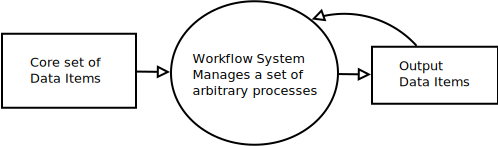
\includegraphics[scale=0.34]{figures/basic_system.pdf}
		\end{center}
		\caption{Basic System Overview}
		\label{intro:basic}
	\end{figure}

	\noindent The system would starts with a
	core set of input files. The workflow is then executed, which initiates a set
	of topologically-sorted tasks. These tasks would then be executed in order, such that
    the processes then generate the full set of output data items. These output items can then
    be used as input files in remaining tasks.

    These processes can be ordered into two main categories:
    \begin{inparaenum}[(i)]
        \item tasks that can automatically be executed by the system; and
        \item tasks that need to be completed by a user.
    \end{inparaenum} The system aims to coordinate an automate these tasks to
    the maximum extent possible whilst managing the information.

    Executing these processes involves using various software packages.
    This functionality can not be replaced by the system so it would need
    to be integrated in a very general way, this would be done by using wrapper
    software software that would use these applications to complete the required goal.

\section{System Evaluation}
    In order to determine the applicability of the proposed solution, the system
    was evaluated in the following ways:

    \begin{description}
        \item[Partial Integration Case Study]\hfill \\
            In order to determine whether the proposed system
            would be applicable to the problem at hand, a portion of the workflow
            of an existing site was implemented and tested within the system. This
            test provides a means to determine whether the problem could be solved
            by the proposed system.
        \item[User Experience Testing] \hfill \\
            Even the most effective system can fail if it cannot
            be successfully be adopted by users. Therefore, the system's
            user experience was tested. This allowed problems to be detected and
            shortcomings of the system to be identified\cite{tullis2008measuring}.
    \end{description}

\section{Legal and Ethical Issues}
    All the software used in the development of the workflow system
    is either free or open source. If this project were to continue
    or be extended, there would not be any legal issues. The core
    of the system is written using the Django Framework, using Python.
    These are, respectively, licenced by the Django Licence and the PSF
    license. Further tools used during the implementation include Javascript
    which is licenced under the LGPL.
    JQuery, JsPlumb and tablesorter, which are dual licenced the  MIT license
    and GPL, Version 2.

    Further data and information was obtained from the Zamani Project for
    testing the application. Permission was obtained to use this data.

    User testing was also done during the course of the project. For
    this purpose, ethical clearance was granted from the Faculty of
    Science Research Ethics Committee. Access to UCT Students was also
    granted by the Department of Student Affairs.

\section{Report Outline}
    This report outlines the design, implementation and evaluation
    of \emph{Zamani Workflow}, a workflow system that sets out to
    solve the data management problems experienced within the
    Zamani Project. The report starts with a review of the literature in
    Chapter~\ref{chap1}.

    This is then followed by the Design and Implementation of the system
    in Chapter~\ref{chap2}. The considerations for the design are defined
    before the full system design is reported. This design process involved
    three iterations.

    The final system in then evaluated in Chapter~\ref{chap3}. This was accomplished
    using a \emph{User Experience} evaluation and an \emph{Integration Case Study}

    The report is then concluded in Chapter~\ref{chap4} where the system is
    reviewed. Here possible future avenues of research is discussed that could
    be used to build on the project.



\chapter{Background\label{chap1}}
    Workflow management systems define a complex process in terms well-defined
    tasks and coordinate process completion \cite{1245778}.  Automated
    workflow management has been in wide use across various disciplines since
    the concept was formalised in 1996\cite{springerlink:10.1007/BF00136712}.
    Successful systems have been implemented across various, fields including
    banking and pharmaceuticals
    \cite{Brahe:2007:SWW:1316624.1316661,5407993}.

    It has been shown to be very successful in the sciences as the same scientific
    process can easily be repeated on a different set of data\cite{4721191}.
    This not only aids in reproducibility but also saves time.  This is done by
    efficiently abstracting the operations in the flow, allowing it to be
    automatically handled.

    Geomatics is the field that concerns itself with the organisation,
    representation and processing of geographic data, for the purpose of
    querying it and making decissions off of the data
    \cite{DiMartino:2007:TAG:1341012.1341081}. The workflow in Geomatics is
    very distributed and the set of data that is operated on is large and
    diverse.  Workflow management within Geomatics has been considered and
    solutions have been proposed, but not implemented or
    evaluated\cite{Migliorini:2011:WTG:1999320.1999356}. 
 
    This chapter presents a discussion on Workflow Systems. Firstly presenting
    an overview of what these systems are and briefly looking into the histories
    of these systems. This is followed by a review of the factors that have influenced
    the success an failure of theses systems.

    Section~\ref{geo:data} does a review of the data and processing involved within
    the field of Geomatics. 

    This is then followed in Section~\ref{example:sys} by a review of existing implementations
    of Workflow Management Systems namely: Kepler, Trident and Taverna. A variety of Case Studies
    ar presented in Section~\ref{casestudy}.



\section{Overview}
A workflow management system consists of definitions on how a set of tasks
should be executed \cite{springerlink:10.1007/BF00136712,vanderAalst2002125}.
The overall procedure is defined by the following components:
\begin{inparaenum}[(i)] \item actors, \item roles, \item responsibilities and
obligations, \item tasks, \item activities,\item conceptual structures and
\item resources.\end{inparaenum}

A real life problem or task can then be broken up into these components in
such a way that the tasks represent a flow network. These tasks then connect to
the actors and resources via the other
components\cite[p.~4]{Taylor:2006:WES:1196459}.  This allows tasks to be
executed efficiently in a distributed manner.

The initial implementations of a workflow system, however, almost
immediately failed. The systems were too rigid and was unable to accommodate the
high levels of change that was required by the users
\cite{Suchman:1983:OPP:357442.357445}.

These changes come from a number of sources, including: ill-specification
of initial problems, change in actors or resources, exceptions that occurred
and new requirements.  Adaptive workflow systems were proposed to solve this
problem by providing a mechanism for allowing change in the
system\cite{vanderAalst2002125}. This allows processes to be extended, replaced
or re-ordered. It also adds the ability to change already running tasks by
providing restart, transfer and proceed options.

Scientific workflow management has also been very successful with how
experiments are defined, and, more importantly, reused. Another benefit that was
quickly discovered was that it also allowed researchers to trade workflows,
making the replication of results much easier than they were
previously\cite{4721191}. Keys to this success were: that the workflow systems
were made to fit the researchers; quick responses to adding required features
when needed; listening to user input and making sharing of workflows as easy as
possible.

Such a system has also been applied in fields that operate on large data
sets, as would be the case if applied to problems in Geomatics  Workflow systems were found to
work well in the management of getting this data processed. Applying the
concept to Observational Astrophysics, it revealed that it could be used to
identify bottlenecks that could be optimised \cite{Aragon:2009:WMH:1529282.1529491}.  Further, it was used to
automatically ensure local access of large files that needed to be processed.


\section{Geographic Data\label{geo:data}}
Geomatics concerns itself with the collection, organisation and query of
geographic data \\  \cite{DiMartino:2007:TAG:1341012.1341081}.  This data includes
but  is not limited to landscapes, coordinate data, building models,
statistics, pictures, textures and routes. This is a very broad set of data,
varying from very large to very small.  That variation, however, means that
there exists no uniform method to efficiently deal with the data.

The processing of this data can vary from human to software processing
\cite{DiMartino:2007:TAG:1341012.1341081}.  Various Web applications have been
written to facilitate the tasks that need to be accomplished.  This software is
known as WebGIS and is becoming more popular with scientists; it also means
that even within the field there is a strong shift toward Web-based services.

A key realisation with the usage of this data is that the same data is used
across various applications, to create various amounts of
abstractions\cite{ElAdnani:2001:MLF:512161.512177}.  The core data is seldom
changed. Instead a new abstraction layer is added on top of it. The data can be
thought of as a graph, where the nodes represent either a data or abstraction
element, and the edges represent the functions/tasks required to create the
particular abstraction as a set of topological relationships. 

\section{Implementations\label{example:sys}}
There are various products available that can compose scientific workflows.
\emph{The Trident workbench} \cite{Simmhan:2009:BTS:1673063.1673121} is an open
source workflow management system developed by Microsoft Research that also
adds middleware services and a graphical composition interface. Trident builds
workflows of control and data flows, off of built-in, user defined activities
and nested subflows.
The flows are represented using XOML, an XML Specification, while the
activities are stored as a set of sub-routines\cite{Simmhan2011790}. Trident
can be used on a local system, remote systems and even clusters.  Queries on
the system can be performed using LINQ.


\emph{Kepler} is another scientific workflow management system that
provides workflow design and execution.  Actors are designed to perform
independent tasks that can either be atomic or  composite
\cite{Wang:2009:KHG:1645164.1645176}.  Composite actors(subflows) consist of
multiple   atomic actors bundled together. Actors can consume data and produce
output, called tokens. Actors communicate tokens with each other via links. The
order of execution and the links are defined by an independent entity called
the director. As a consequence, the workflow can either be executed in a
sequential or parallel manner. Kepler effectively separates the workflow from
its execution, allowing for easy batch execution. Actors can easily be exported
and shared.  Kepler is very popular due to its adaptability and easy
integration.

    \emph{Taverna} is a scientific workbench that supports application-level
workflow and does not focus on scheduling as much as others\cite{4721191}. Taverna
has a strong focus on workflow sharing. Taverna is quite popular, since there
exists a social network designed to facilitate workflow sharing among
scientists(\emph{myExperiment}). Services are linked to the model to execute
the various tasks. Taverna can be used in such a way that it can utilize all
the services a client has to facilitate the flow by easily adding services. The
Taverna language is a simple data-flow language called the Simple Conceptual
Unified Flow Language(SCUFL), that can be encoded in XML.

In order for these workbenches to be successful, there needs to exist a
high level of interoperability between the workflow management and the services
that are required \cite{Shegalov:2001:XWM:767132.767139}.  However, due to the
fact that there is a relatively high chance of failure when building this
interoperability into the services as a core component. It is an extremely high
risk and therefore is not typically done. A cheaper way of doing this is
providing middleware that can wrap around the service to provide the required
interfaces.

This need for interoperability has led to the popularisation of SOA(Service
Orientated Architecture) \cite{Sanders:2008:SSA:1400549.1400595}.  It should be
noted that SOA is \emph{not} an implementation, but rather an
\emph{Architectural Model}; SOA refers to a collection of loosely coupled
services, that individually carry out a particular process. Each service should
have a well defined interface with self-contained functionality. It should
allow other applications or services to use this functionality without knowing
the underlying technical details. These services should be hidden from the
end-user and their usage should preferably be platform-independent.

Although the concept has been around since the 1970s, it has only recently
gained favour due to Web services.  Web services are software components that run on the
Internet through XML standards-based
interfaces\cite{Tai:2004:CCW:1045658.1045680}.  Each service provides a
functional description using the \emph{Web Services Description Language}(WSDL).
This description provides the supported operations, as well as the definition
of the input and output messages.

By using these concepts, a workflow system can be built that automatically uses
these Web Services to facilitate both the data and control flow using well-defined
interfaces in standards such as XML/JSON \cite{Shegalov:2001:XWM:767132.767139}. 
With the advancement of WebGIS, a lot
of Web Services that facilitate Geomatics processing already exist.


\section{Case Studies\label{casestudy}}
The next section will look at two instances where workflow management systems
were implemented and used.  These case studies will look at both a business and
a scientific application.
    \subsection*{Danske Bank}
      The workflow management system at \emph{Danske bank} was incrementally
      implemented as their system moved from a manual
      system\cite{Brahe:2007:SWW:1316624.1316661}.

      This system was developed as an in-house solution when the manual system
      could not cope any longer.  Several lessons were learnt that are applicable
      to other workflow systems. When work was divided purely from an
      efficiency point of view, the workers became complacent as they felt that
      they did not understand the overall mechanism and felt that they were not
      involved. They discovered that the system did not handle change very
      well. This change was expensive and inevitable. Their system had to be
      adapted to handle this change. The success of the system is mainly
      attributed to the interoperability and close relationship between the
      users and the developers

    \subsection*{OrthoSearch}
      \emph{OrophoSearch} is a workflow, built on \emph{Kepler}, that is
      designed to work on data in the field of Bioinformatics.
      \cite{daCruz:2008:OSW:1363686.1363983}

      A workflow system was implemented in \emph{Kepler} as it addressed the
      requirements they had, including: \begin{inparaenum}[(i)] \item workflow
      definition and design; \item workflow execution control; \item fault
      tolerance; \item intermediate data management; and \item data provenance
      support.  \end{inparaenum}

      Although the system was not without its hiccups and changes, the
      integration with Kepler provided the workflow with increased overall
      productivity.

    \subsection*{Sunfall}
      \emph{Sunfall} is a workflow system that was created to assist in locating
      supernovas from large amount of telescope data\cite{Aragon:2009:WMH:1529282.1529491}.
       
      Sunfall consists of four components: \begin{inparaenum}[(i)]\item Search, \item 
      Workflow Status Monitor, \item Data Forklift and \item Supernova Warehouse.\end{inparaenum} 
      
      The Search component is responsible for coordinating the tasks responsible for 
      coordinating tasks involved in finding supernovas, within the data. The system
      is also tasked with dealing with an enormous amount of data, up to 100TB. The
      data movement is carried out using the \emph{Data Forklift} component.

      This project used a Parallel File system, to aid in data replication within the
      project and used middle ware to interface with legacy software.

      Sunfall was deemed a great success as it not only successfully improved the
      efficiency and identified bottlenecks within the process


\section{Summary}
This chapter reviewed the appropriate literature for Workflow Management Systems
and the data variety and processing within Geomatics. This has provided the necessary
insight to determine what components would be required in order to build such a Workflow
System for the Zamani Project.

The process to create the heritage artifacts from the raw-scans and photographs
generates a large amount of varied data. A Workflow Management System would need
to be able to specifically cater for this constraint similarly to the large scaled
data involved in the implementation of both \emph{OrthoSearch} and \emph{Sunfall}.


Since the tasks are however a mixture between automated and manual tasks. Such a
system would be able to map to a more grid-based approach and was shown to be done
at \emph{Danske Bank}. Middleware would need to be provided in order for the system 
to uniformly integrate with applications required throughout the process\cite{Montella:2007:UGC:1272980.1272995}.
The model has been shown to be able to be effectively automated using a Workflow Management System\cite{Withana:2010:VWE:1851476.1851586}. 


\input{design}

\chapter{Evaluation\label{chap3}}

For the system to be successfully utilized within the project
it needs to accomplish the following goals:
\begin{enumerate}
\item It needs to be able to integrate the daily tasks of the users
      without it being a burden.
\item It needs to effectively  manage the data items and
      coordinate the tasks between the users and the system.
\end{enumerate}

In order to answer these questions, the system needed to be evaluated on two
fronts. \emph{User Experience} evaluations were performed to test whether the
system could be easily adopted by users if implemented.

The system was then tested further to see if it could perform
a subset of the tasks it would be required to perform if implemented within
the \emph{Zamani Project}. Due to time constraints, the entire set of task required
to support the activities of the Zamani Project could not be implemented.

\section{User Experience Evaluation}
Users and their experience of a system is becoming a critical component
in designing a software system\cite{Forlizzi:2004:UEI:1013115.1013152}.

User Experience evaluations aim to understand the needs and experiences of a user.
In order to do this, user engagement needs to be tested on both a visual and emotional level.
These evaluations are used to link the needs of the users to the functionality provided by the
system. The benefit gained from having a usable system is that the productivity
of the users is greatly increased\cite{nielsen2003usability}.
User Experience experiments were performed to ensure that the system
provides a good, usable interface.

\subsection{Aim}
The aim of the usability test is to assess the quality of the system. This
assesses the user's ability to complete required tasks efficiently while
remaining satisfied with the system\cite{bevan1995measuring}. This is done in
order to determine how suitable the solution is for the user.

The usability of the system was be rated using the following attributes
\cite{doi:10.1207/s15327590ijhc1803_3}:
\begin{description}
\item[Learnability] Relates to the capability of the software to enable a user
    to learn how to use it. This is a goal for the system as this would
    enable users to quickly start using the software effectively.
\item[Efficiency] Refers to the time it takes for the
    user to complete a certain goal or task.
\item[Satisfaction] Measures the attitude of the users towards software. This
    includes: \begin{inparaenum}[(i)]\item Difficulty;\item Confidence; and
        \item Like/Dislike towards the system\end{inparaenum}.

\item[Error] Number of errors that a user makes, including deviations from
    the intended path.
\item[Effectiveness] This tests user efficiency based on a predetermined level
    in terms of speed, number of errors and steps.
\item[Simplicity] Amount of effort that is required for a user to complete a
    task. This can be traced in terms of number of selections or time taken to
    search for a function.
\end{description}

To measure the user experience, a simple performance evaluation is not
enough. We need to be able to gain insight on how users feel about the system
\cite{vermeeren2010user}. This requires that the emotional state of the user be
evaluated.

\subsection{Methodology}
In order to determine the attributes mentioned above, a quantitative \emph{User Experience}
 experiment was set up. Users were asked to complete two task using
the system. The system was designed to support a workflow. This involves two main
user activities: \begin{inparaenum}[(i)] \item Management of individual tasks;
and \item Setting up workflows \end{inparaenum}. The tasks were designed to test
these operations. Their experiences were recorded and then evaluated. The detailed
process is outlined below.

\subsubsection{Task Setup}
Tasks were set up for users to complete. The aim of these tasks was to simulate
the main activities of the system. This led to the formalisation of two tasks
that are described as follows:
\begin{description}
\item[Complete a set of tasks as a user] \hfill \\
    The first part was to simulate the actions of an unprivileged user
    who is required to do outstanding tasks.  A Site was created containing three
    tasks. These tasks were assigned to the test user. Since the system aims to
    support tasks that are executed on the user's workstation, the tasks were
    designed to be as simple as possible. Since the general usability of the system
    was to be evaluated, the tasks were not related to processing digital cultural
    artifacts.

    Three \emph{Python} programs were set up to represent the user tasks
    that were to be executed. For \emph{Task one} and \emph{Task two},
    the user was simply required to run the desktop application. The third
    task, however, aims to test the user's understanding of the system by
    asking the user questions about the task. These questions are:
    \begin{inparaenum}[(a)] \item What is the output directory for the
    task?;  and \item Please select the input files that are used in this
    task\end{inparaenum}?   The task descriptions all convey what the purposes
    of the tasks are. As soon as the user completes a task, they need to
    indicate on the system that the task has been completed.
\item[Build a simple workflow] \hfill \\
    For the second part the user had to simulate the role of a privileged
    user, and had to set up a sample workflow. The tasks represent a workflow
    that produces a PDF file starting with a text file. This was given as a
    diagram to the users. The diagram can be seen in Figure~\ref{eval:workflow}.
        The user was given very little instruction on how to complete the task.
    This allows them to explore the system and intuitively complete the task.

\end{description}
\begin{figure}[!h]
    \begin{center}
        \includegraphics[scale=0.45]{figures/workflow.png}
    \end{center}
    \caption{Workflow that needed to be recreated}
    \label{eval:workflow}
\end{figure}
To ensure that each user experienced the system the same way, it was restored to
its previous state after each test.

\subsubsection{Questionnaire}
The primary method used to evaluate the \emph{User Experience} of the system was
using a questionnaire. Questionnaires attempt
to obtain the subjective feelings of the user towards the
system\cite{Chin:1988:DIM:57167.57203}. In order to measure the experience, the
emotional response of the user also has to be obtained. The USE questionnaire
was chosen to evaluate the User Experience \cite{lund2001measuring}. This
questionnaire is designed to determine the usability attributes in terms of:
\begin{inparaenum}[(i)]\item Usefulness;\item Ease of Use; \item Ease of learning; and \item
Satisfaction \end{inparaenum}. It is designed in such a way that an
emotional response is triggered. In order to avoid \emph{Acquiescence Response Bias},
the questionnaire duplicates responses in such a way that the they were
phrased both negatively and positively.
In order to save on paper, the survey was conducted using \emph{Lime
Survey}\footnote{Lime Survey: http://www.limesurvey.org/},
The questionnaire used can be found in Appendix~\ref{appendix:questionnaire}.

\subsubsection{Monitoring and Pilot Tests}
During the tests the users were monitored and their actions noted. This was to
determine what the overall process was for each of the users. All
questions, actions and errors were also noted during this process. These events
were noted by time to produce the remaining usability attributes namely:
\begin{inparaenum}[(i)]\item Efficiency; \item Error; \item Effectiveness; and \item
Simplicity  \end{inparaenum}

After the tasks were set up, the user tests were run using two users. This was
used to determine problems that would adversely affect the results before it was
run using a larger test group. The results of the pilot test identified some
minor issues regarding how the questions were worded, that distracted the users
from the task at hand. This was fixed before the full tests were conducted.

\subsubsection{User Selection}
The participants chosen for the user experiment were not the users that would
be interacting with the system on a daily basis. This is to avoid confirmation
bias that is likely to occur due to the fact that they are stakeholders in the
project\cite{kaptchuk2003effect}. 

The participants varied in age ranging from 18 to 24. Due to cost and time
constraints all subjects tested were students. The level of
technical competence varied from novice to expert. The students were highly
diverse in terms of \emph{Field of Study}, being drawn from four faculties:
Economics, Engineering, Science, and Humanities. 24 participants were used 
to perform the evaluation.

\subsection{Results}
The user evaluation produced a number of results. Users were on average able to
finish the task $21$ minutes, with an interquartile width of
$7$ minutes. This indicates that the users were mostly able to complete the task
in the expected time. All but one user was able to complete the
entire set of tasks that were provided. Results of the test were acquired using two
methods: the survey; and the data from the observations.

The survey independently measured data for both tasks that the participants were
required to execute. This aimed to get the users' opinions on the categories
regarding: \begin{inparaenum}[(i)] \item Usefulness; \item Ease of use; \item
Ease of Learning; and \item Satisfaction \end{inparaenum}. Values with a high
amount of variance were not considered to be significant.\\

\subsubsection{Execute Simple Tasks}
The participants were asked to evaluate their experiences with regard to
completing the tasks. The survey, along with the observations was used to
rate the experience in terms of the following categories:
\begin{description}
    \item[Usefulness] \hfill \\
    	Overall, the users found that the system was useful and allowed them to be
    	productive. There is a general indication that the system was well
    	equipped to support the tasks that were executed by the participants.
	$76\%$ of participants found the system useful.

    	From observation it seemed that users were easily able to use the system
    	to indicate the tasks. There appeared to be very little confusion as to
    	what the purpose of the buttons on the interface was.

    	There was a slight delay, for about $30\%$ of users, between the
	completion of the first task and
    	when the users started the second task since the task screen displayed
    	either that \emph{data was being transferred back} or that the task
    	was \emph{awaiting validation}. They seemed to wait for the system to
    	indicate that the status has changed, without realising that the
    	validation process was manual. This reduced the initial usefulness of
    	the system, prompting that more interactive task reporting is possibly
    	required.
    \item[Ease of use] \hfill \\
    	The number of steps required to complete the task was considered to be
    	minimal by $80\%$ of the users, and very few inconsistencies were
	noted. $71\%$ of participants agreed that the system was easy
	and simple to
    	use. The system was described as flexible and users were able to
    	recover from mistakes easily.

    	It should be noted that participants initially found the concept of
    	specifying \emph{input files} and the \emph{output folder} while
    	completing \emph{Task $3$} confusing. $50\%$ of users had to be told
    	what the task was asking. From the user responses, this can likely be
    	attributed to phrasing of \emph{Task $3$} within the system.

    \item[Ease of Learning] \hfill \\
        The system was described as being very easy to learn by  $90\%$ of
    	participants. They found that the system was very easy to remember.
    	$75\%$ of users described themselves as somewhat skilful after using
	it for a short	period of time.

    	This corresponds with the observations made during the test. Since
    	participants were given no instructions on how to use the system, they
    	were initially quite hesitant to perform actions. However, as the
    	experiment moved along, their actions became much faster and more
    	decisive.

     \item[Satisfaction] \hfill \\
        $85\%$ of participants were satisfied with the experience
	with the system and that it allowed
        them to complete the tasks with relative ease. Users emotionally
        responded to the system in the following way: \begin{inparaenum}[(i)]
    	\item it was pleasant to use; and \item that the system was
        wonderful\end{inparaenum}.

        Some users showed clear signs of satisfaction when they started getting
        used to the interface. At no point did any of the participants appear
        frustrated while completing the first part of the experiment.

    \item[Efficiency] \hfill \\
        The efficiency of the survey was not measured by the survey and all
        findings are based on the observations of the users. Users took an
        average time of $7$ minutes in completing the first task. The slowest
        time taken was $12$ minutes. The interquartile range was determined
        to be between $5$ minutes and $8$ minutes, showing that most of the
        users were able to efficiently accomplish the tasks provided.

        Some efficiency issues were noted in the hesitance of participants
        after completing the first task, before starting the second task.
        This could be attributed to the participants being unfamiliar with the
        system; however it is an indication that better task feedback would
        likely increase efficiency.
\end{description}
Overall, the task interface yielded positive results on the \emph{User
Experience} of the system. Layout issues were identified that caused users
to navigate to unexpected places, but users were quickly able to recover from
this without needing assistance. The learnability tests showed that the system
was very easy to learn and it required very little effort on the part of the
participants to use it successfully.

\subsubsection{Build Simple Workflow\label{eval:simple}}
For this task the participants were asked to build a simple workflow, that had
been provided on a diagram. (See Figure~\ref{eval:workflow}) The instructions
did not provide any information on how the system should be used and
participants were required to determine how to complete the task on their own.
\begin{description}
\item[Usefulness] \hfill \\
    $85\%$ of participants indicated that they found the system to be
    effective for the task that was required. $80\%$ also indicated that
    the system aided them in being productive and completing the task.
    Overall, $94\%$ of users found the system useful.

    Users found that the system gave them good control over what they were doing and
    made the task relatively easy to complete, and felt the number of steps
    involved were appropriate.

    Observations of the participants revealed that the participants quickly
    understood what was expected and were able to use the system to
    effectively build the workflow that was required. All users were able to
    complete the task.
\item[Ease of Use] \hfill \\
    $85\%$ of participants indicated that they found the system simple and easy to use.
    They believed that the number of steps were minimal to complete the tasks
    that were required. Inconsistencies within the system was not noted by
    the participants. $75\%$ of users felt like they were easily able to recover after
    making an error. They were confident that the system was being used
    successfully. In addition, $75\%$ of users commented very favourably on
    ease of use.

    While monitoring the user interaction, users navigated the entire page before
    deciding on how they would add a task. Typically they would select the
    \emph{User Task} and be confused that the option for the \emph{Server Task}
    was  not available. Several users were directed to the cancel button. This
    indicates that the option should be combined and indication as to what the
    task type is should appear in the combobox.

    Users did seem to intuitively understand that the tasks could be dragged
    within
    the visualisation. Furthermore, since the creation of a task placed the node
    in a fixed position in the visualisation, users seemed to believe that their previous task
    had been overwritten. Stronger visual cues on the nodes in the visualisation
    should be added to indicate that drag options are available. Nodes should
    also initially be randomly placed to avoid confusion. A similar problem was
    noted in dragging the \emph{arrow icon} to indicate dependencies.

    A rather significant problem was encountered during the testing. While
    the users were navigating the page to determine what to do, they encountered
    the Jobs section, believing this is where they needed to add tasks. This
    wasted a lot of time for some users. This is caused by the confusing
    terminology that was used. Better naming convention should be established to avoid
    this problem.
\item[Ease of Learning] \hfill \\
    Users were very quickly able to determine how the system worked and how to
    use it efficiently. Participants grew much more confident and decisive as
    the task progressed. This is also validated by $85\%$ of the responses in
    the survey, indicated that the system was very easy learn.
    Participants did not hesitate between tasks and quickly added all the
    required nodes.
\item[Satisfaction] \hfill \\
    $90\%$ of users were very satisfied with the system; and $57\%$ agreed
    that the  system was fun to use.
    Participants felt that the system worked the way
    they expected it to work. Emotional responses, that give a better indication of the user
    experience, indicated that a significant portion of the users believed the
    system to be wonderful and that they need to have it. Overall, $80\%$
    users found
    the system pleasant to use.

    During the experiment, the users were noted to express excitement and
    happiness was expressed when they realised how the system works.


\item[Efficiency] \hfill \\
    Users took an average of $7$ minutes to complete, with an interquartile range
    of $5$ to $9$ minutes. Once the participants had placed the first task, they
    were immediately more efficient. The efficiency of the participants was
    quite varied. Some participants spent a significant amount of time
    staring at the visualisation, as they thought that the previous tasks had
    been removed, due to the \emph{drag-and-drop} functionality not being
    apparent.
\end{description}

\noindent The second task was overall rated as a positive experience; while some participants
expressed the need for more complete instructions, on using
the system. However, based on the data acquired on the \emph{learnability} of the
system, this appears to have been the appropriate choice. The experiment strongly
indicated that the \emph{Job} terminology would need to be reworked. Further
observations showed that more visual cues are required to indicate that the
tasks notes are \emph{draggable}.

The user study was able to highlight problems associated with the system. These
include: \begin{inparaenum}[(i)]\item Task Feedback; \item Navigation; \item
Visual cues; and \item certain Terminology\end{inparaenum}. In terms of
usability criteria, \emph{Effectiveness} and \emph{Simplicity} could not be
tested due to resource and time constraints. Findings on the usability were as
follows:

\begin{description}
\item[Learnability] Users were very quickly able to get used to the system and
	became competent in completing the tasks.
\item[Efficiency] Participants were able to complete the tasks in the required
	amount of time. This was done intuitively without giving specific
	information on how to use the interface.
\item[Satisfaction] Users indicated that they were satisfied with the system. It
	was also noted that overall the participants were not frustrated with
	the system. Users confidently used the system and did so with ease.
\item[Error] Participants who did make errors were able to recover swiftly
	using the interface. Problems however did arise with the job terminology
	where users were confusing jobs with tasks, causing errors. Some detours
	were also noted where a group of participants were not able to
	intuitively navigate back to the \emph{Task Overview} screen.
\end{description}



\section{System Test}
The system needs to be evaluated in terms of its applicability to successfully 
manage and coordinate the tasks of the Zamani Project.
 Due to time constraints, however, the full set of the tasks within the project
could not be implemented. In order to evaluate its applicability,  two tests were
 performed to test whether the  solution would work. The first test was designed to
determine the general applicability of such a system, by executing a workflow that
is unrelated, while the second test involves implementing small portion of the tasks
of the Zamani Project to determine if if could be successfully implemented.

\subsection{Applicability Tests}
Two test were performed. The first test was to build a simple workflow that
creates a document. The second test builds a workflow that represents a portion
of the process that creates a 3D model from the raw scan.




\subsubsection{Creating Document}
The purpose of this task is to mix user tasks along with server tasks. This
workflow is the same workflow that was used in the user test. A representation
of the workflow can be seen in Figure~\ref{eval:workflow}.
The process involves: a user creating a ``\emph{.txt}'' file. Images are then
converted to a different format. These are then converted to the \LaTeX~format
with the pictures added. The document is then compiled to a \emph{PDF}.

The workflow was successfully able to build the document. The completed workflow
can be seen in Figure~\ref{eval:document}.

\begin{figure}[!h]
    \begin{center}
        \includegraphics[scale=0.45]{figures/document_test.png}
    \end{center}
    \caption{Completed workflow that creates a simple PDF document}
    \label{eval:document}
\end{figure}

\subsubsection{Integration Test}
A lengthy process is requires to build the 3D models from the initial laser scans require a lengthy
process. This process can be illustrated in Figure~\ref{eval:zamani}
\footnote{Source: Zamani Project at UCT}.
 In order to test whether the system can be applied successfully, a portion of this process
was implemented in the system.

\begin{figure}[!h]
    \begin{center}
        \includegraphics[scale=0.65]{figures/zamani_workflow.pdf}
    \end{center}
    \caption{Zamani - 3D Modelling Workflow}
    \label{eval:zamani}
\end{figure}
The first five steps in the modelling process were implemented using the workflow
system to determine how the system would support running on actual data. Since
data from a previous site was available, the user tasks were merely simulated
by copying over the required data for this task. This was implemented
successfully. Figure~\ref{eval:zamani_impl} shows the workflow being executed.

\begin{figure}[!h]
    \begin{center}
        \includegraphics[scale=0.45]{figures/zamani_impl.png}
    \end{center}
    \caption{Partially implemented Zamani modelling workflow}
    \label{eval:zamani_impl}
\end{figure}

\noindent This successful integration shows that the system is able to support some
workflows required by the Zamani project.


\subsection{Filtering}
The system can successfully implement the workflow required for the Zamani
Project, however filtering workflow at a site level is not ideal. Many workflows
get replicated at a building level and beyond this the artifact creation can
also be distinguished by category. In order for the workflows built within the
system to be more reusable, it would need to be extended to store workflows at
finer level. These could then be nested in a hierarchical manner. This would
allow entire workflows to be abstracted as a single node. This would decrease
set up time and increase reusability of the system, however, further
experimentation would be required to determine the effect on User Experience.

\subsection{Performance}
The movement and processing of data is regarded as being the most expensive
portion of the process. The data movement is directly offloaded to \emph{rsync},
whereas the data processing is offloaded to the native applications. The system
management of these activities outperforms these tasks. As such, the system's
performance is bounded by these activities. This offloading procedure is
illustrated in Figure~\ref{eval:offload}.

\begin{figure}[!h]
    \begin{center}
        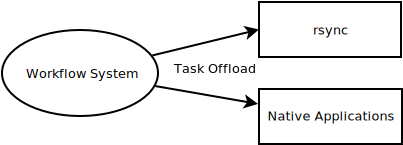
\includegraphics[scale=0.45]{figures/offload.pdf}
    \end{center}
    \caption{Performance: Task offload}
    \label{eval:offload}
\end{figure}

Due to this, a performance evaluation of the system was not deemed necessary.
Performance of the system could, however, be affected by several processes being
executed simultaneously. In order to speed up the process in this case the
system would need to be distributed to include multiple processing servers; this
was decided outside the scope of the project.

\section{Summary}

The system was evaluated and it was determined that: \begin{inparaenum}[(i)] \item
it can successfully integrate a portion of the Zamani Workflow; and \item user could
successfully use the system with very little effort.\end{inparaenum} The terminology was found
to be somewhat confusing and it was found that better filer filtering options would be
beneficial. Overall, however, the system was evaluated as being a success.



\chapter{Conclusion and Future Work\label{chap4}}

This system can successfully manage a complex set
of tasks with arbitrary dependencies. Tasks could be either be fully automated
by the system or could be completed by users. When user tasks are started, the
required files are incrementally transferred to the desktop host of the user
using \emph{rsync} to only transfer files that have not been transfered or are
out of date. To enforce quality and accuracy, a feature was added that enforces
that user tasks be validated by experienced members of the team before the tasks
can be labelled as complete.

Automated tasks are executed on the
server due to the fact that these tasks operate on very large files. By executing
them locally, data does not need to be transferred, which would be an expensive
process. Tasks are automatically started when all dependencies are met.

In the event that a task fails, the system also allows the user to inspect the
logging information that is generated during the execution of the task. Once the
problem is identified the tasks can then be manually restarted.

\section{Conclusion}
This research project was concluded with the successful implementation of a
Workflow Management System.  The design and
implementation was done in three iterations. This was explained in depth in
Chapter~\ref{chap2}.


The system was then successfully evaluated in Chapter~\ref{chap3} both for its
usability and its effectiveness at solving the problem. The following positive
results was obtained during the evaluation of the system:
\begin{enumerate}
    \item The system was successfully able to implement and execute a portion of
        the workflow in the modelling section of the modelling tasks that are
        present in the Zamani-Project. This sample workflow used a mix of system
        and user task.
    \item The system was positively evaluated using a sample group of 24 users.
        This evaluation revealed that users found the system useful, easy to
        use and users were satisfied using the system. User responses and the
        observations made during the test it was found that the system is
        effective and is very easy to learn.
\end{enumerate}

This system was however not implemented within the production Zamani Project. This was
mainly due to time constraints, caused by the scale and time required to
implement it. Functionally the system could be implemented, however this process
could be significantly simplified by the addition of some features. These are
mentioned in the future work session.


\section{Future Work}
During the implementation of the workflow system, various possible extensions
that could be added to the system could
not be implemented. These features would improve the system both in terms of
performance,
usability and set up time.
\begin{description}
\item[Hierarchical Workflows]\hfill \\
To allow better control and re usability over tasks, workflows should be
abstracted to include a hierarchy. Such a hierarchy would allow entire workflows
to be represented as singular nodes. These workflow, could then be repackaged
and reused in different sites, or even the same site. This would also allow the
setup for new sites to be much faster, as prepackaged workflows could easily be
used as drop-in components.
\item[Parameterized Scripts]\hfill \\
Oftentimes particular parameters of a script can change from one site to
another. This change does not necessarily affect the \emph{Task type}; however,
with the current implementation of the system the change would need to be made
at this point. This can be greatly improved by allowing a \emph{Task} to send
parameters to the job. This would require the Task Subsystem to allow parameters to
be sent dynamically to the \emph{Task Type}.
\item[Rule Based File Filters]\hfill \\
Currently within the system all the files in the output directory of are task is
treated as input to successor tasks. Tasks often only use a portion of the
files created by the predecessor. In order to currently facilitate this with the
system an additional filtering, task would need to be set up that filters out
unused files. By including a rule based filtering system much greater control
can be placed on the output files. Such rule based filters have been
successfully implemented in other systems\cite{conery2005rule}.
\item[Interactive Task Feedback Options]\hfill \\
In order to avoid one of the problems that were found in Section~\ref{eval:simple},
more interactivity is required for \emph{Tasks}. This primarily includes
real-time updates on the status of tasks. Further developments include the
ability to do more interactive validation such as discussion integration.
The addition of these collaborative tasks could resolves issues
with tasks in a uniform manner\cite{guimaraes1998integration}.
\item[Transformation-based Task Support]\hfill \\
Currently the system is built around creating derivative data items. However, it
is often common for certain files within a site to change, without creating an
additional copy. Although this behaviour is implicitly allowed, it should be
extended to be better defined within the system.
\item[Parallel Task Processing] \hfill \\
One of the most crucial aspects affecting the long term feasibility of the
system is its ability to scale and handle larger and more complicated workflows.
In this regard the server node would become a significant bottleneck in
processing \emph{Server Tasks}. In order to alleviate this problem, the system
would need to become distributed. This would present its own set of problems
as data would need to be efficiently distributed along the computation nodes
to ensure efficiency.

\end{description}





\bibliography{bibliography}{}
\bibliographystyle{apalike}
\appendix
\includepdf[pages=-,picturecommand*={%
     \put(42,760){%
              \parbox{\textwidth}{\chapter{Questionnaire}\label{appendix:questionnaire}}
	      }}]{survey.pdf}


\end{document}
